% Editable native annotations around unchanged verified IDE photographs.
\par
\begin{figure}[htbp]
\centering
\newsavebox{\MARSwavchunkregistersBox}
\sbox{\MARSwavchunkregistersBox}{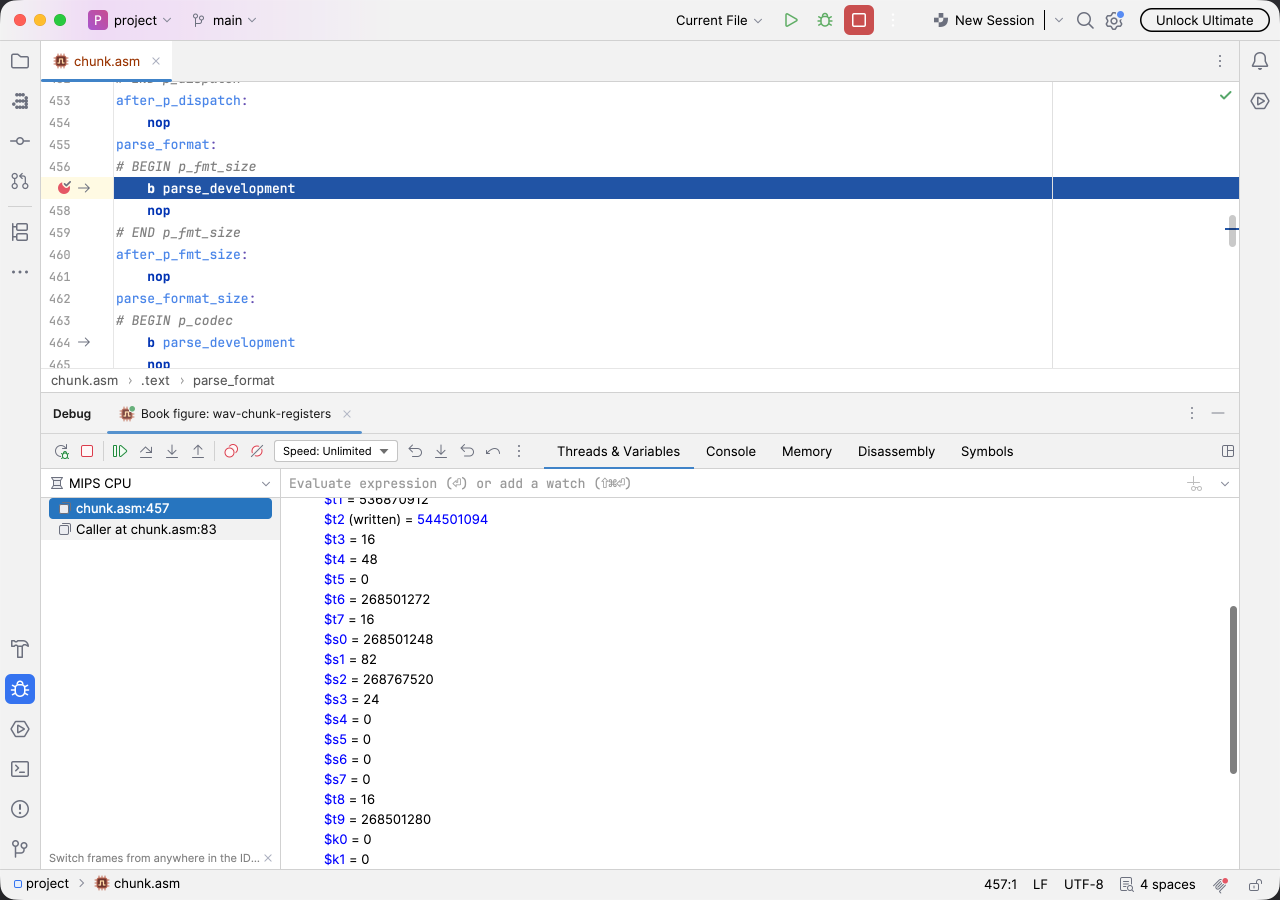
\includegraphics[artifact]{packages/031-pcm-wav/captures/f02/registers.png}}
\newsavebox{\MARSwavchunksourceBox}
\sbox{\MARSwavchunksourceBox}{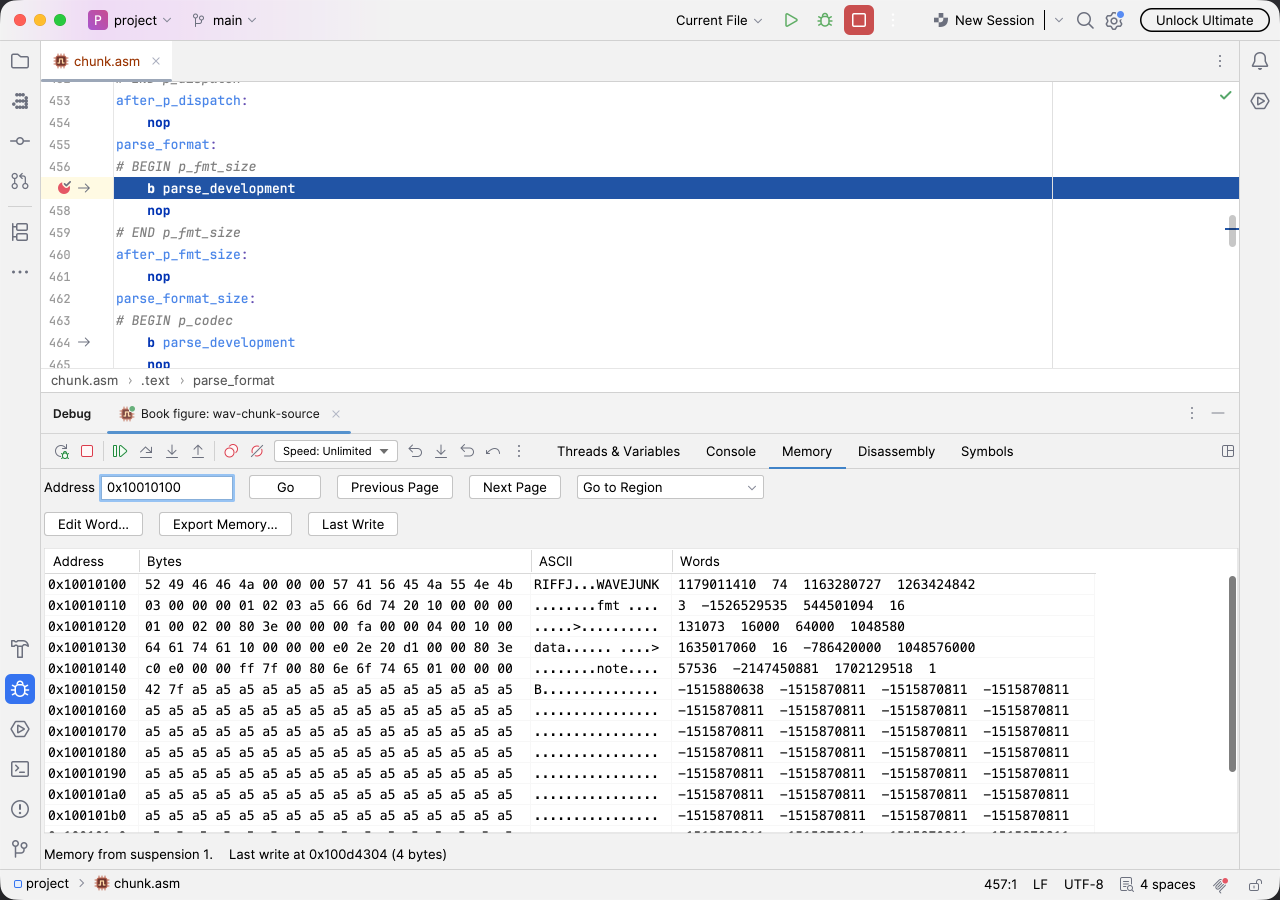
\includegraphics[artifact]{packages/031-pcm-wav/captures/f02/source.png}}
\newsavebox{\MARSwavchunkmetadataBox}
\sbox{\MARSwavchunkmetadataBox}{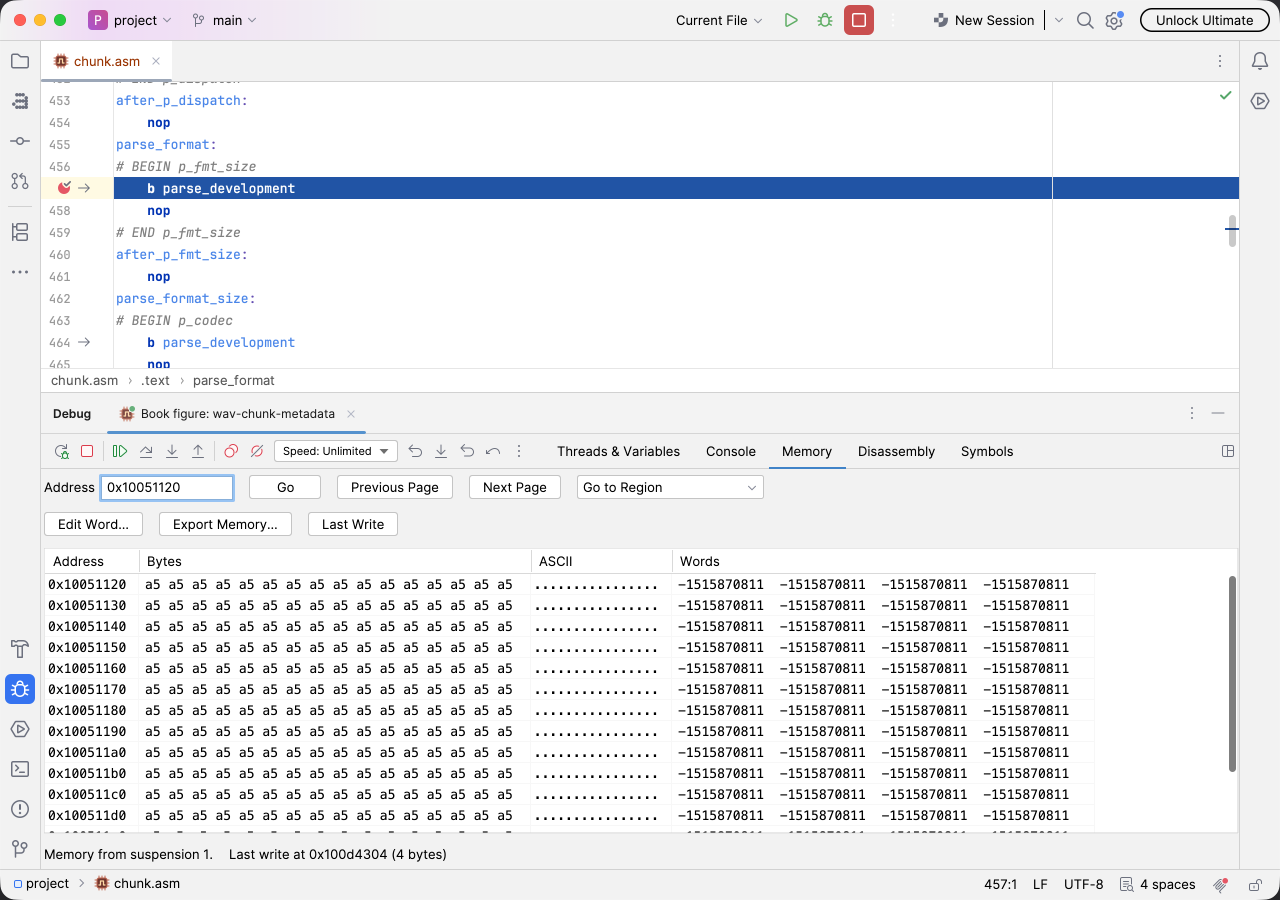
\includegraphics[artifact]{packages/031-pcm-wav/captures/f02/metadata.png}}
\edef\MARSwavchunksourceLeft{\the\dimexpr0.036718750\wd\MARSwavchunkregistersBox\relax}
\edef\MARSwavchunksourceBottom{\the\dimexpr0.774444444\ht\MARSwavchunkregistersBox\relax}
\edef\MARSwavchunksourceRight{\the\dimexpr0.713281250\wd\MARSwavchunkregistersBox\relax}
\edef\MARSwavchunksourceTop{\the\dimexpr0.170000000\ht\MARSwavchunkregistersBox\relax}
\edef\MARSwavchunkcursorLeft{\the\dimexpr0.246093750\wd\MARSwavchunkregistersBox\relax}
\edef\MARSwavchunkcursorBottom{\the\dimexpr0.211111111\ht\MARSwavchunkregistersBox\relax}
\edef\MARSwavchunkcursorRight{\the\dimexpr0.553906250\wd\MARSwavchunkregistersBox\relax}
\edef\MARSwavchunkcursorTop{\the\dimexpr0.763333333\ht\MARSwavchunkregistersBox\relax}
\edef\MARSwavchunklengthLeft{\the\dimexpr0.246093750\wd\MARSwavchunkregistersBox\relax}
\edef\MARSwavchunklengthBottom{\the\dimexpr0.100000000\ht\MARSwavchunkregistersBox\relax}
\edef\MARSwavchunklengthRight{\the\dimexpr0.553906250\wd\MARSwavchunkregistersBox\relax}
\edef\MARSwavchunklengthTop{\the\dimexpr0.874444444\ht\MARSwavchunkregistersBox\relax}
\edef\MARSwavchunkinputLeft{\the\dimexpr0.034375000\wd\MARSwavchunksourceBox\relax}
\edef\MARSwavchunkinputBottom{\the\dimexpr0.287777778\ht\MARSwavchunksourceBox\relax}
\edef\MARSwavchunkinputRight{\the\dimexpr0.584375000\wd\MARSwavchunksourceBox\relax}
\edef\MARSwavchunkinputTop{\the\dimexpr0.608888889\ht\MARSwavchunksourceBox\relax}
\edef\MARSwavchunkmetadataLeft{\the\dimexpr0.034375000\wd\MARSwavchunkmetadataBox\relax}
\edef\MARSwavchunkmetadataBottom{\the\dimexpr0.311111111\ht\MARSwavchunkmetadataBox\relax}
\edef\MARSwavchunkmetadataRight{\the\dimexpr0.584375000\wd\MARSwavchunkmetadataBox\relax}
\edef\MARSwavchunkmetadataTop{\the\dimexpr0.608888889\ht\MARSwavchunkmetadataBox\relax}
\begin{tikzpicture}[alt={Five details at parse_format show the next unfinished instruction, header offset 24, payload length 16, the JUNK payload 01 02 03 followed by pad a 5, the next fmt header and unchanged caller metadata.}]
\node[anchor=north west,inner sep=0,font=\small\bfseries] (source-title) at (6mm,0) {Before accepting the format payload};
\node[anchor=north west,inner sep=0] (source) at ([yshift=-1mm]source-title.south west) {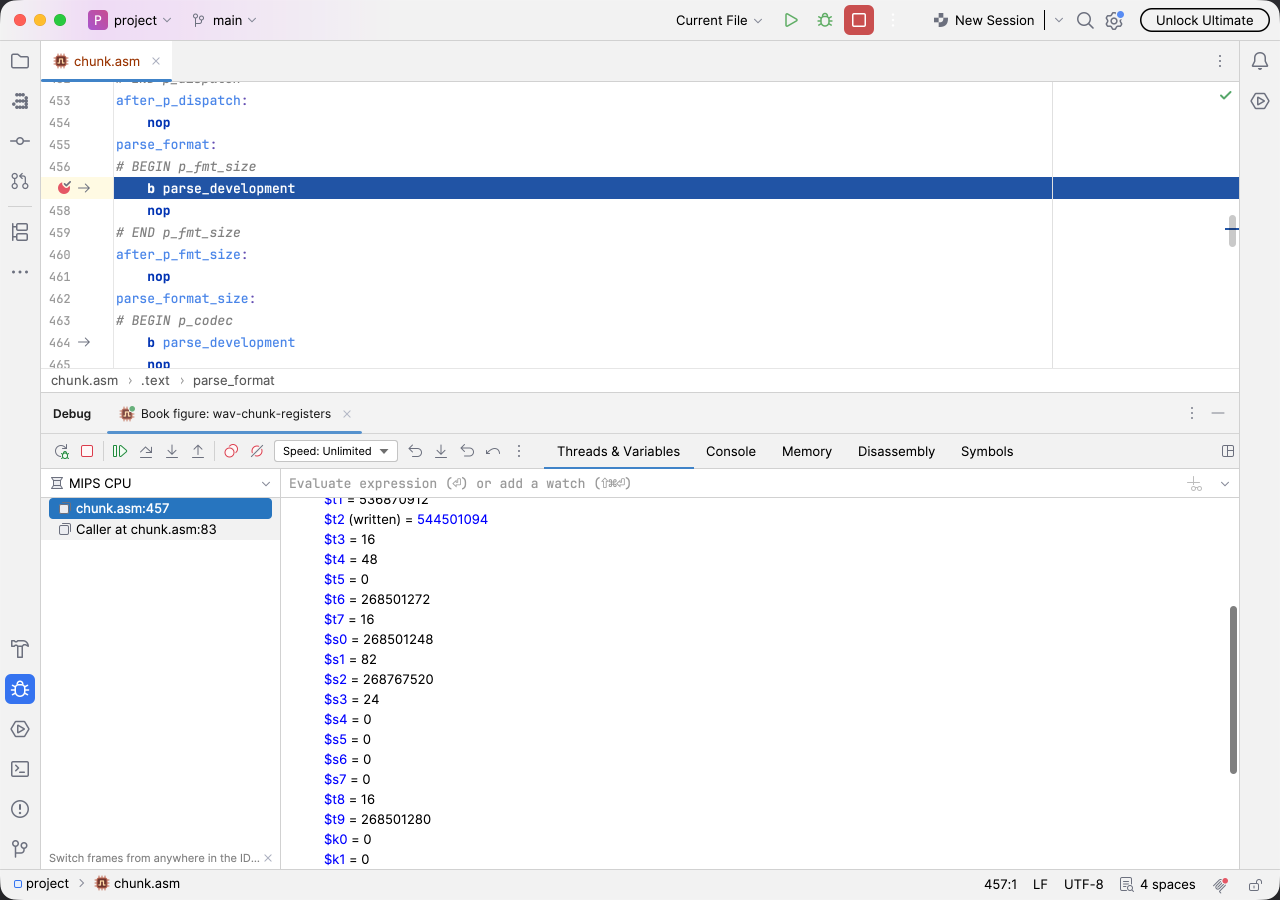
\includegraphics[width=0.54\linewidth,artifact,trim={\MARSwavchunksourceLeft{} \MARSwavchunksourceBottom{} \MARSwavchunksourceRight{} \MARSwavchunksourceTop{}},clip]{packages/031-pcm-wav/captures/f02/registers.png}};
\begin{scope}[shift={(source.south west)},x={($(source.south east)-(source.south west)$)},y={($(source.north west)-(source.south west)$)}]
\draw[black,line width=0.7pt] (0.215625000,0.080000000) rectangle (0.775000000,0.520000000);
\node[draw=black,fill=white,circle,inner sep=1.5pt,font=\footnotesize] at ($(0.215625000,0.520000000)+(-3mm,0)$) {1};
\end{scope}
\node[anchor=north west,inner sep=0,font=\small\bfseries] (cursor-title) at ([yshift=-1mm]source.south west) {Current header offset};
\node[anchor=north west,inner sep=0] (cursor) at ([yshift=-1mm]cursor-title.south west) {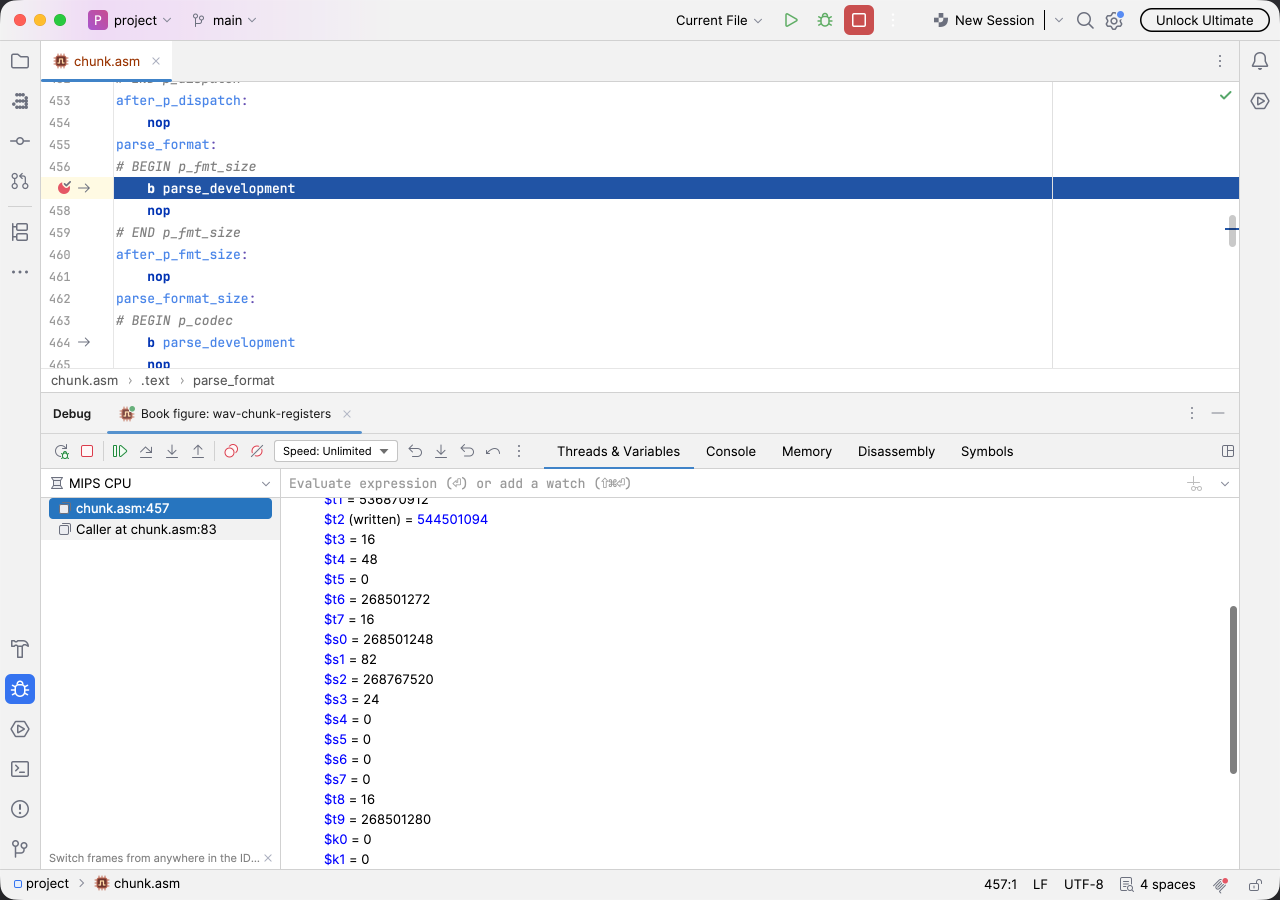
\includegraphics[width=0.44\linewidth,artifact,trim={\MARSwavchunkcursorLeft{} \MARSwavchunkcursorBottom{} \MARSwavchunkcursorRight{} \MARSwavchunkcursorTop{}},clip]{packages/031-pcm-wav/captures/f02/registers.png}};
\begin{scope}[shift={(cursor.south west)},x={($(cursor.south east)-(cursor.south west)$)},y={($(cursor.north west)-(cursor.south west)$)}]
\draw[black,line width=0.7pt] (0.023437500,0.043478261) rectangle (0.257812500,0.913043478);
\node[draw=black,fill=white,circle,inner sep=1.5pt,font=\footnotesize] at ($(0.023437500,0.913043478)+(-3mm,0)$) {2};
\end{scope}
\node[anchor=north west,inner sep=0,font=\small\bfseries] (length-title) at ([yshift=-1mm]cursor.south west) {Format payload length};
\node[anchor=north west,inner sep=0] (length) at ([yshift=-1mm]length-title.south west) {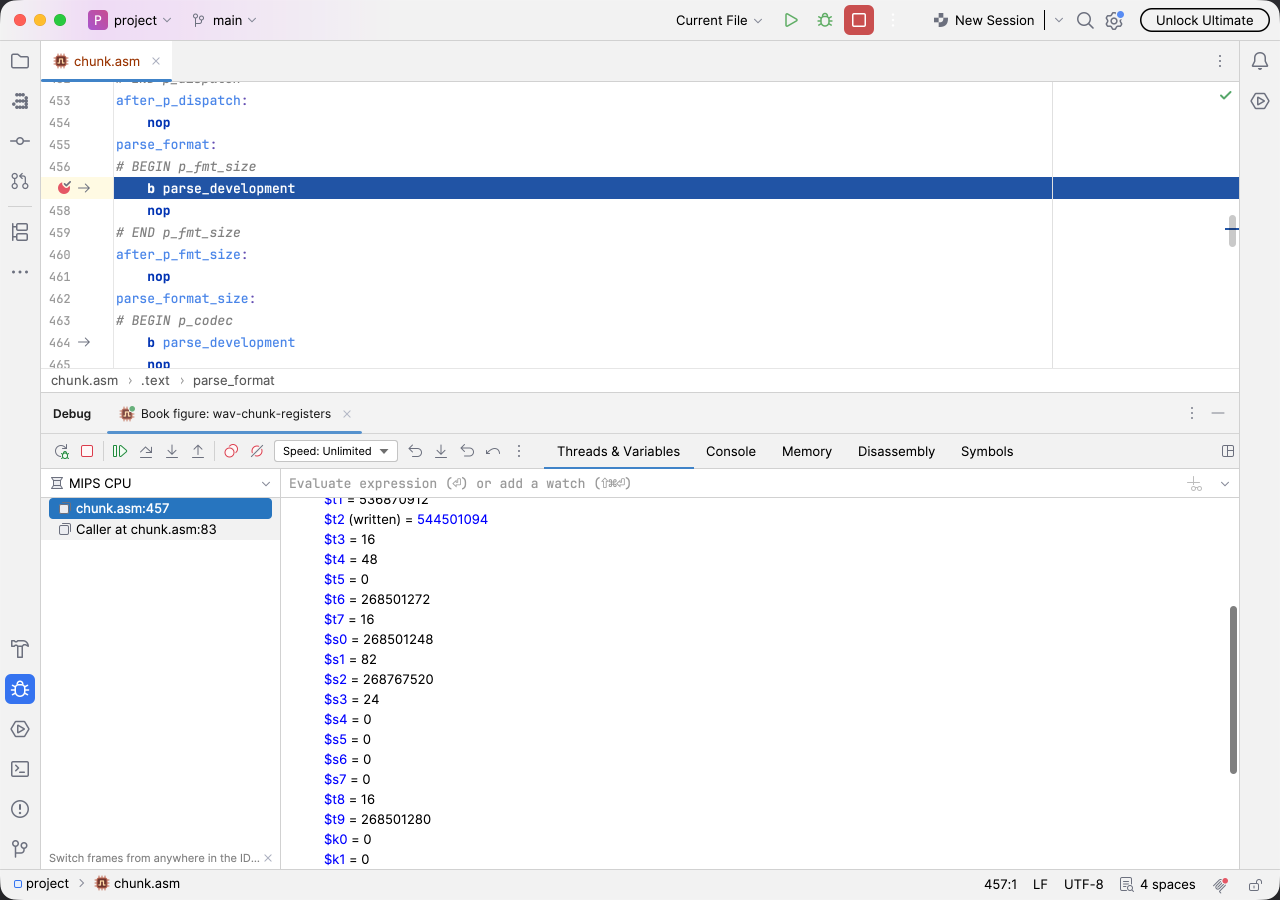
\includegraphics[width=0.44\linewidth,artifact,trim={\MARSwavchunklengthLeft{} \MARSwavchunklengthBottom{} \MARSwavchunklengthRight{} \MARSwavchunklengthTop{}},clip]{packages/031-pcm-wav/captures/f02/registers.png}};
\begin{scope}[shift={(length.south west)},x={($(length.south east)-(length.south west)$)},y={($(length.north west)-(length.south west)$)}]
\draw[black,line width=0.7pt] (0.023437500,0.043478261) rectangle (0.242187500,0.913043478);
\node[draw=black,fill=white,circle,inner sep=1.5pt,font=\footnotesize] at ($(0.023437500,0.913043478)+(-3mm,0)$) {3};
\end{scope}
\node[anchor=north west,inner sep=0,font=\small\bfseries] (input-title) at ([yshift=-1mm]length.south west) {Container bytes through the format payload};
\node[anchor=north west,inner sep=0] (input) at ([yshift=-1mm]input-title.south west) {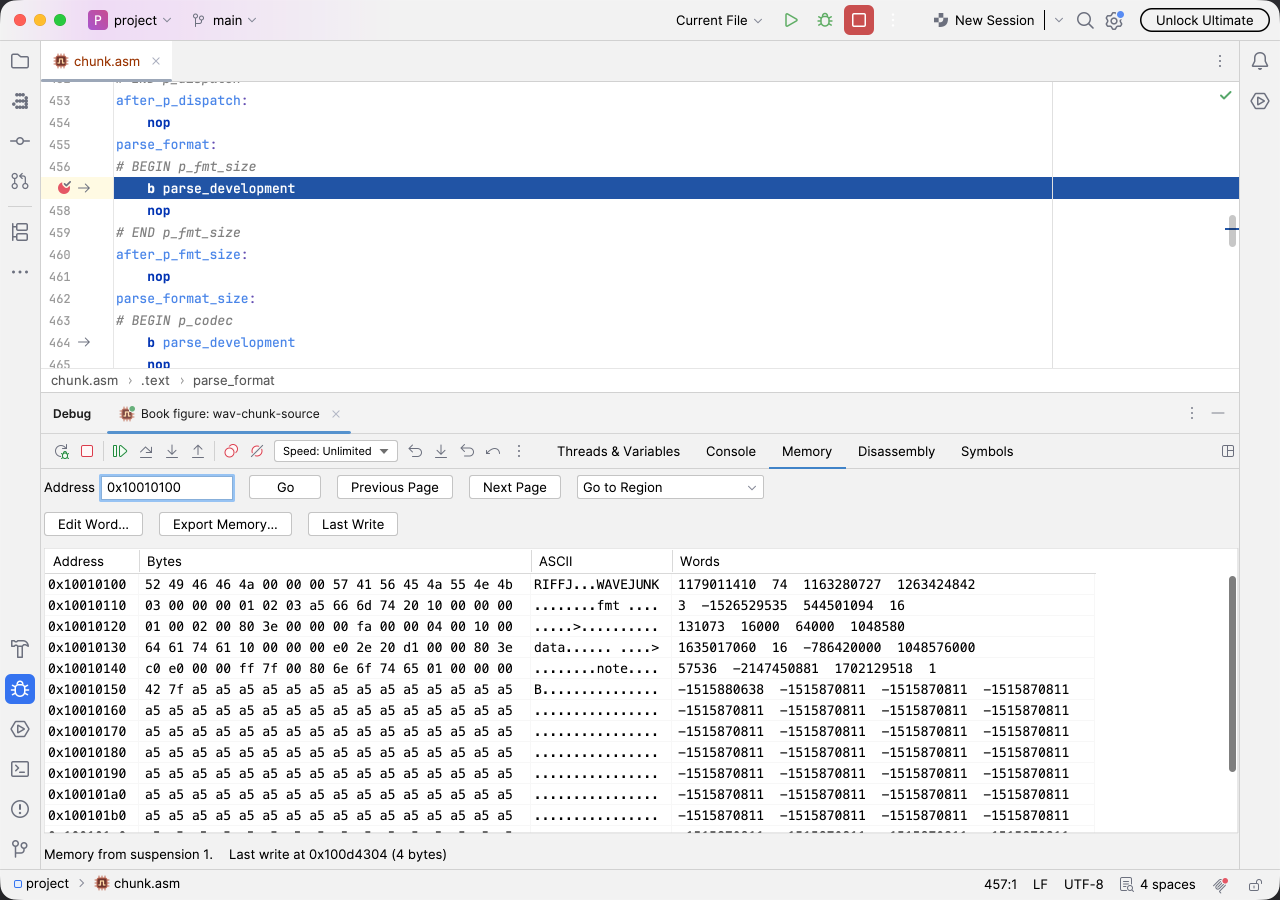
\includegraphics[width=0.84\linewidth,artifact,trim={\MARSwavchunkinputLeft{} \MARSwavchunkinputBottom{} \MARSwavchunkinputRight{} \MARSwavchunkinputTop{}},clip]{packages/031-pcm-wav/captures/f02/source.png}};
\begin{scope}[shift={(input.south west)},x={($(input.south east)-(input.south west)$)},y={($(input.north west)-(input.south west)$)}]
\draw[black,line width=0.7pt] (0.194672131,0.043010753) rectangle (0.997950820,0.720430108);
\node[draw=black,fill=white,circle,inner sep=1.5pt,font=\footnotesize] at ($(0,0.720430108)+(-3mm,0)$) {4};
\end{scope}
\node[anchor=north west,inner sep=0,font=\small\bfseries] (metadata-title) at ([yshift=-1mm]input.south west) {Caller descriptor before publication};
\node[anchor=north west,inner sep=0] (metadata) at ([yshift=-1mm]metadata-title.south west) {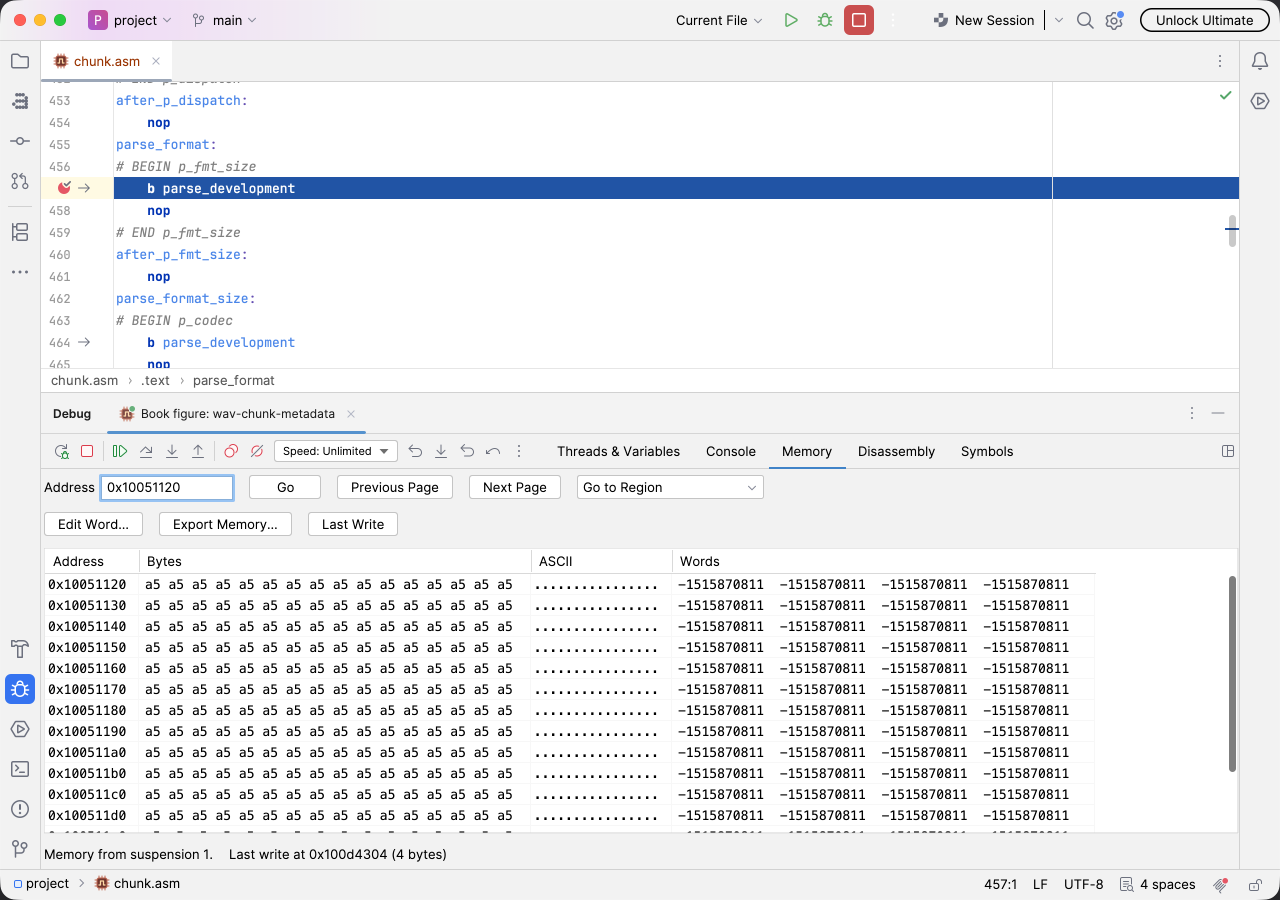
\includegraphics[width=0.84\linewidth,artifact,trim={\MARSwavchunkmetadataLeft{} \MARSwavchunkmetadataBottom{} \MARSwavchunkmetadataRight{} \MARSwavchunkmetadataTop{}},clip]{packages/031-pcm-wav/captures/f02/metadata.png}};
\begin{scope}[shift={(metadata.south west)},x={($(metadata.south east)-(metadata.south west)$)},y={($(metadata.north west)-(metadata.south west)$)}]
\draw[black,line width=0.7pt] (0.194672131,0.055555556) rectangle (0.997950820,0.638888889);
\node[draw=black,fill=white,circle,inner sep=1.5pt,font=\footnotesize] at ($(0,0.638888889)+(-3mm,0)$) {5};
\end{scope}
\end{tikzpicture}
\par\smallskip
\begin{minipage}{\linewidth}
\small
\begin{enumerate}
\setlength{\itemsep}{0pt}
\setlength{\parsep}{0pt}
\item Execution is stopped before the first instruction at \texttt{parse\_format}. This is the cumulative step-eleven program: format validation has not yet been authored.
\item \texttt{s3 = 24} locates the current header relative to the source base. The earlier JUNK chunk occupies eight header bytes, three payload bytes and one pad byte, so the next header starts at $12+8+3+1=24$.
\item \texttt{t8 = 16} is the current format payload length. This length excludes its eight-byte header. Keep payload length, padded span and next header offset distinct.
\item The row starting at source offset sixteen contains the JUNK length, payload \texttt{01 02 03}, pad \texttt{a5}, and the next identifier \texttt{66 6d 74 20} (\texttt{fmt }). The pad must exist within the container; this profile does not require its value to be zero.
\item The caller metadata remains \texttt{a5}. Finding a format header does not publish a description. Continuing this partial program reaches development status four at the unfinished format region.
\end{enumerate}
\end{minipage}
\caption{An odd-sized opaque chunk ends with a pad before the next header.}
\label{capture:031-pcm-wav-f02}
\label{pcm-wav-f02}
\end{figure}
\par
